%!TEX root = ../main.tex;
\chapter{Le Web sémantique}
\label{annexe:semantic-web}
% TODO appendix parts

% What is semantic web?

% Le Web tel que nous le connaissons aujourd'hui est encore conforme
% à la vision initiale.

% Le Web a été conçu principalement pour une utilisation par les
% humains. Néanmoins, il existe un effort visant à automatiser son
% utilisation et d'être plus accessible pour les machines.

% \cite{bartalos2011effective} The Web was primarily designed for use
% by humans. Nevertheless, there is an effort to automate its use
% and bring the Web more accessible for machines. This has brought
% forward the need for machine processable representations of
% semantically rich information. This has brought forward the need for
% machine processable representations of semantically rich
% information: a vision at the heart of the Semantic Web

Dans un premier temps, on va essayer de clarifier la notion d'un
service Web sémantique, puis étudier les langages émergeants qui
permettent de décrire ce type de service Web.

L'objectif premier du Web sémantique est de définir et lier les
ressources du Web afin de simplifier leur utilisation, leur
découverte, leur intégration et leur réutilisation dans le plus grand
nombre d'applications \cite{berners2001semantic}. Le Web sémantique
doit fournir l'accès à ces ressources par l'intermédiaire de
descriptions sémantiques exploitables et compréhensibles par des
machines. En effet, Les technologies du Web sémantique complètent le
Web actuel avec des outils sémantiques. Il ne s'agit donc pas de créer
un nouveau Web ou un Web séparé de l'existant : ce Web de données
repose entièrement sur les technologies et concepts qui ont fait le
succès du Web tel que nous le connaissons aujourd'hui
\cite{bertails2010web}.

La réalisation du Web sémantique trouve ces racines dans le
développement des langages de balises inspiré par des travaux issus
de la communauté AI \cite{mcilraith2001semantic}, tels que \textsc{OIL}
\cite{fensel2001oil}, \textsc{DAML+OIL} \cite{horrocks2002daml+oil} et
\textsc{DAML+OTN} \cite{mcguinness2003daml} (ces deux derniers
langages font partie de la famille \acrshort{daml}).

  % TODO refactor
Ces langages ont une sémantique bien définies et permettent le balisage
et la manipulation des taxonomies complexe et des relations logiques
entre les entités sur le Web. \cite{fensel2000creating}

% %!TEX root = ../main.tex
\begin{figure}[h]
    \centering
    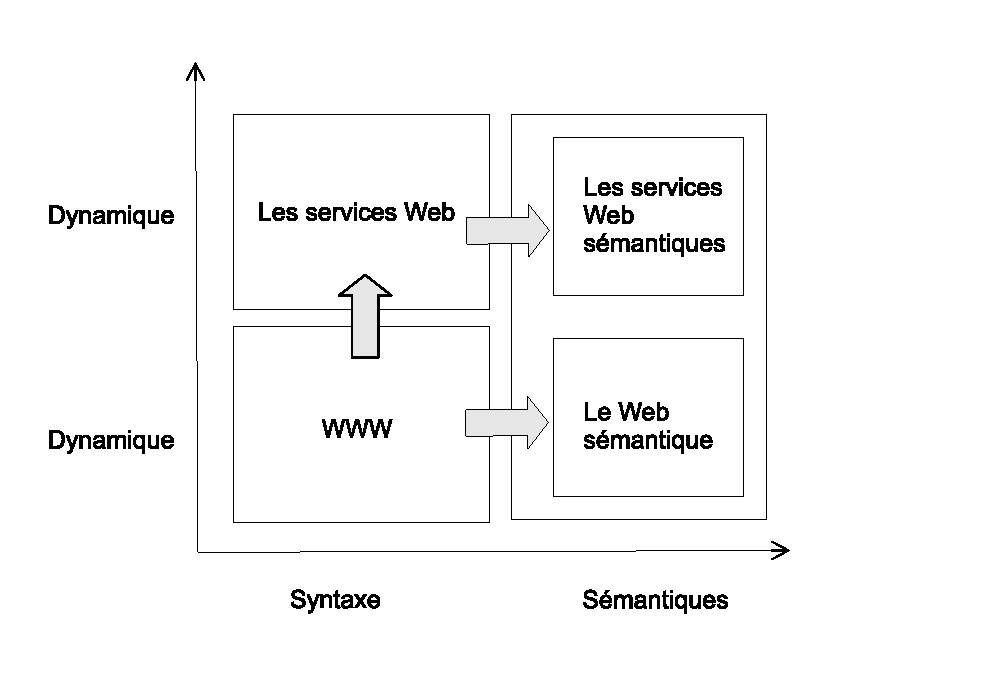
\includegraphics[width=1\textwidth]{figs/3w_to_sws.eps}
    %TODO translate
    \caption{Web evolution to Semantic Web services \cite{fensel2002semantic}.}
    \label{fig:3w_to_sws}
\end{figure}

Cette description repose sur des ontologies. Selon Gruber
\cite{gruber1993translation}, une ontologie est une spécification
explicite d'une conceptualisation. Une conceptualisation est un modèle
abstrait qui représente la manière dont les personnes conçoivent les
choses réelles dans le monde     et une spécification explicite signifie
que les concepts et les relations d'un modèle abstrait reçoivent des
noms et des définitions explicites. Le Web sémantique est devenu un
domaine à part entière, preuve en est la création en 2001 du groupe de
travail sur ce sujet par le \textsc{W3C}.

%%% Local Variables:
%%% mode: latex
%%% TeX-master: "../main"
%%% End: